\normaltrue \difficilefalse \tdifficilefalse
\correctionfalse
%\UPSTIidClasse{11} % 11 sup, 12 spé
%\newcommand{\UPSTIidClasse}{11}

\exer{Système éclipse $\star$ \label{C2:04:65:02}}
% Banque PT SI A 2009
\setcounter{question}{0}\UPSTIcompetence[2]{C2-04}
\index{Compétence C2-04}
\index{Correcteur}
\index{Correcteur avance de phase}
\index{Système éclipse}


\ifcorrection
\else
\marginnote{\textbf{Pas de corrigé pour cet exercice.}}
\fi
\ifprof
\else 

Le schéma-blocs sous la forme suivante avec un gain unitaire pour le capteur
de vitesse.

\begin{center}
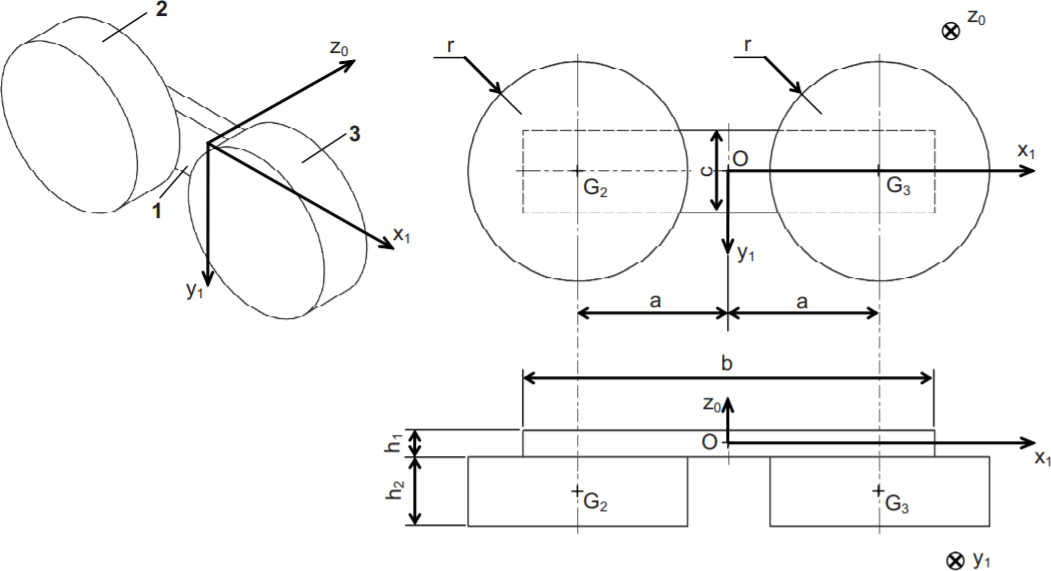
\includegraphics[width=\linewidth]{65_01}
\end{center}

$H_L(p)=\dfrac{K_L}{1+\tau_L p}$ et $H_G(p)=\dfrac{K_G}{1+\tau_G p}$  avec $\tau_G=\tau_L = \SI{20}{ms}$, $K_L = \SI{1e-3}{N^{-1}s^{-1}}$ et $K_G = \SI{2e-5}{mN^{-1}s^{-1}}$.


Le cahier des charges donne les valeurs des critères d'appréciation adoptés :
\begin{itemize}
\item la précision : en régime permanent à vitesse constante, soit $\varepsilon_S=0$ et à accélération constante, soit $\varepsilon_T=0$; $\varepsilon_S$ désigne l'erreur statique de position et $\varepsilon_T$ l'erreur statique de vitesse ou erreur de traînage;
\item la rapidité : le temps de réponse à \SI{5}{\%} tel que : $t_{\text{R}\SI{5}{\%}}\leq \SI{1}{s}$;
\item la stabilité : marge de phase $\geq \SI{45}{\degres}$ et marge de gain $\geq \SI{10}{dB}$.
\end{itemize}

On considère que le système n'est pas perturbé et que $T_G(p)=0$.
On choisit une correction telle que $C_{V}(p)= C_{V1}(p) \cdot C_{V2}(p) $ avec $C_{V1}(p)=\dfrac{K_i}{p^2}$ et $C_{V2}(p)=\dfrac{1+k_f \tau_v p }{1+\tau_v p }$ où $k_f$ est appelé coefficient de filtrage et dont la valeur est généralement comprise entre $5\leq k_f \leq 10$.
\fi

\question{Comment se nomme la correction apportée par $C_{V2}(p)$ ? Expliquer brièvement comment ce type de correction
permet de stabiliser un système instable. Pour cela, tracer l'allure du diagramme de Bode correspondant à ce
terme.}
\ifprof
\else 
\fi


\ifprof
\else 
La figure suivante fournit les diagrammes de Bode du système corrigé uniquement par le correcteur 
$C_{V1}(p)$ avec $K_V=1$, c'est-à-dire la fonction de transfert $W(p) =\dfrac{1}{p^2}H_L(p)$.


\begin{center}
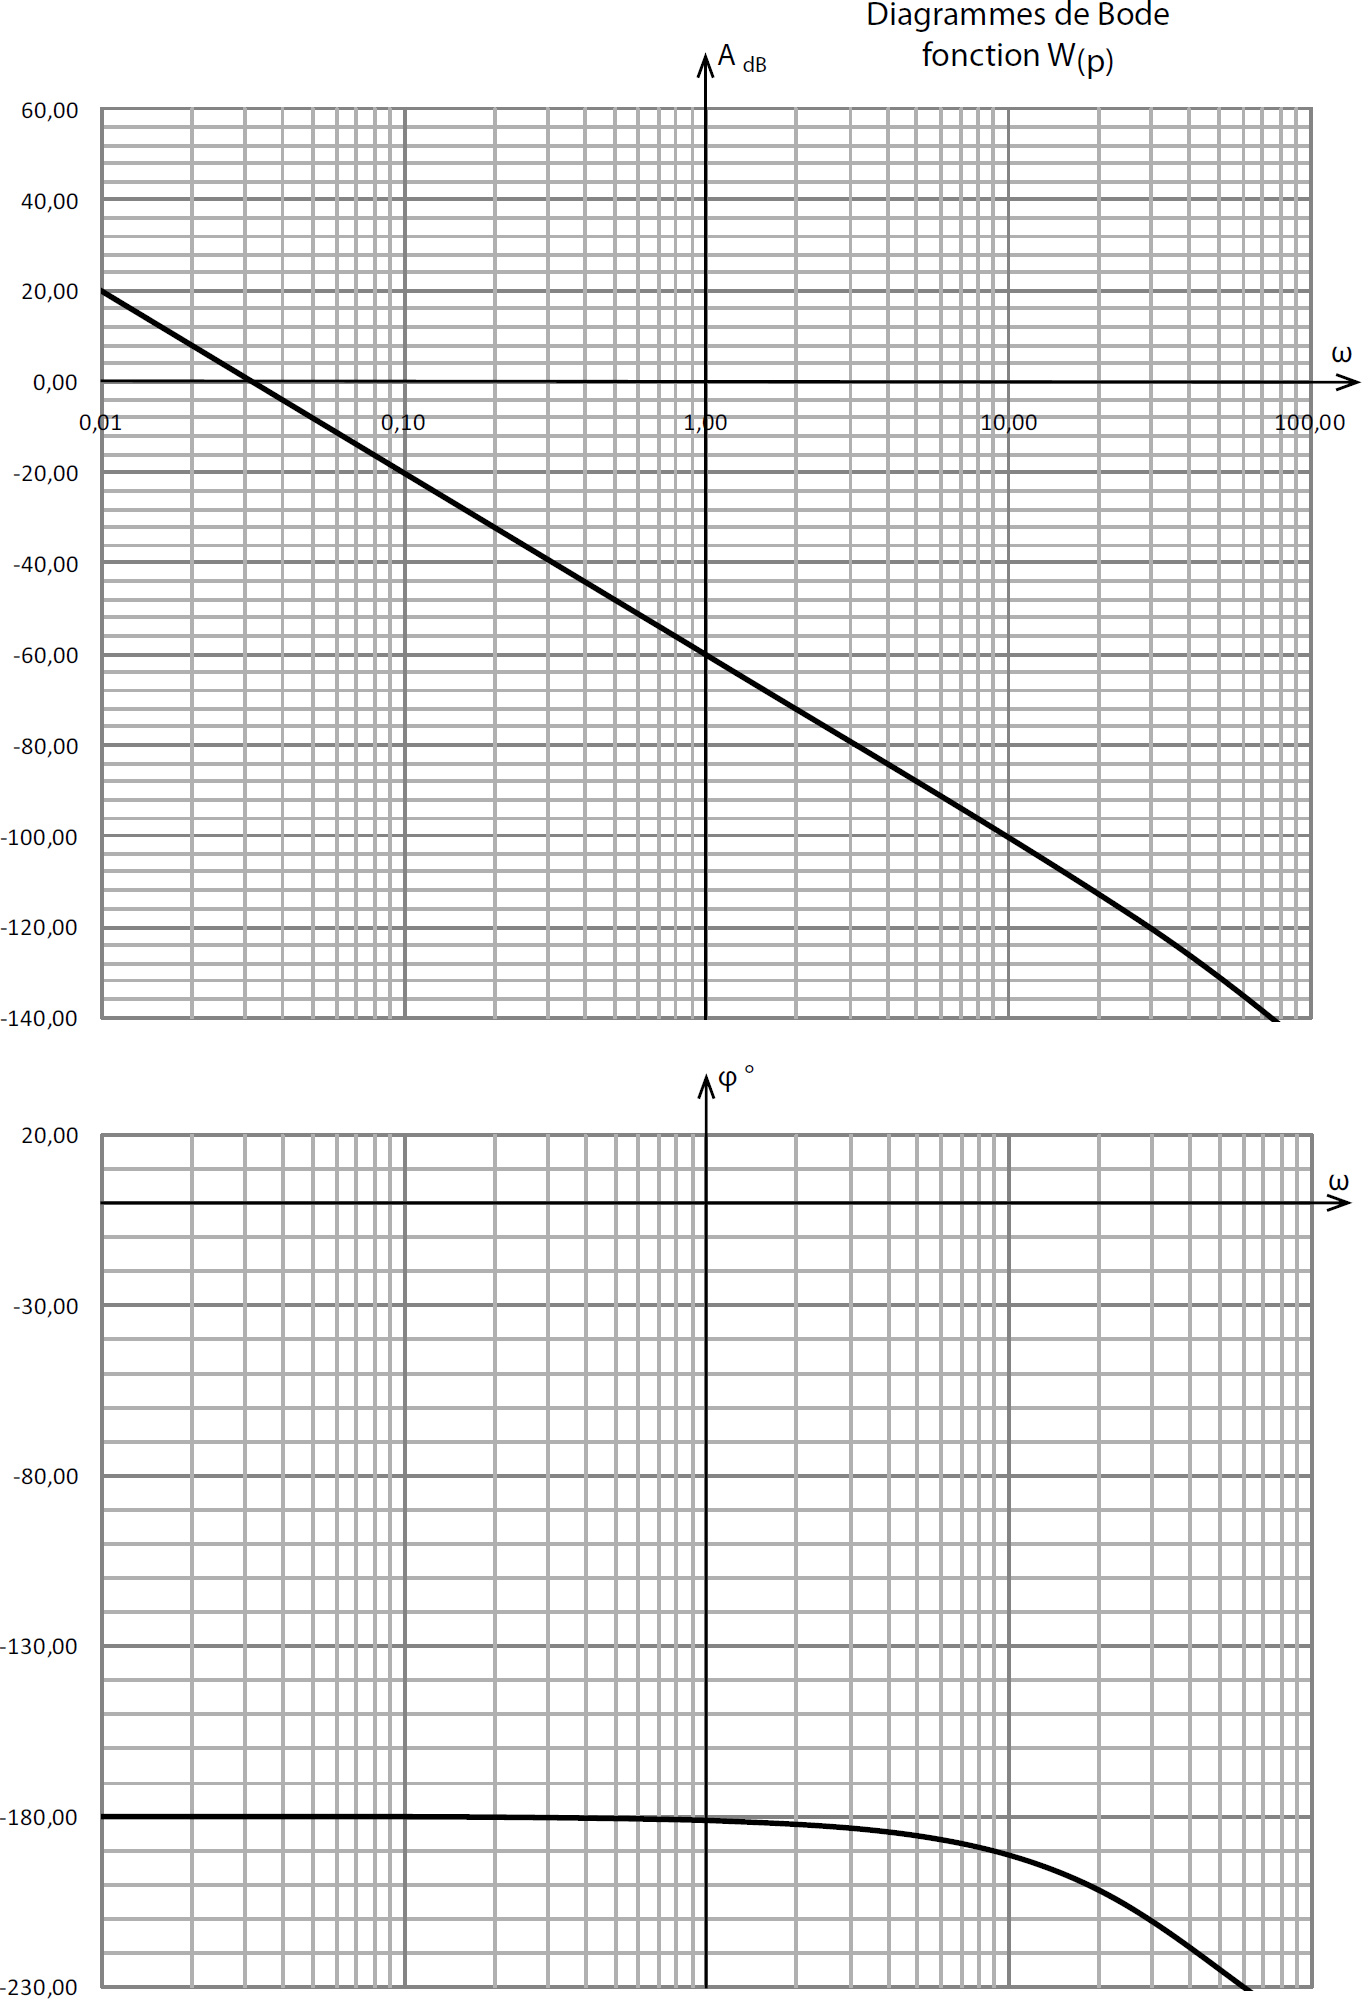
\includegraphics[width=\linewidth]{65_02}
\end{center}
\fi

\question{Lire sur les diagrammes de Bode du système de fonction de transfert $W(p)$, la valeur de la
pulsation de coupure $\omega_{\SI{0}{dB}}$ où le rapport d'amplitude $A_{\text{dB}}$ s'annule. Quelle est, à cette pulsation, la valeur de la
phase ? Justifier alors la présence de la correction $\dfrac{1+k_f \tau_v p }{1+\tau_v p }$}
\ifprof
\else 
\fi

\question{Exprimer en fonction de $\tau_V$ et de $k_f$ la pulsation $\omega_m$ pour laquelle la phase maximale est atteinte. On rappelle pour cela que $\dfrac{\dd \arctan x}{\dd x}=\dfrac{1}{1+x^2}$.}
\ifprof
\else 
\fi

\ifprof
\else 
On montre que pour un coeffcient de filtrage $k_f=8$, la valeur maximale de la phase, ajoutée par la correction,
est de $\SI{51}{\degres}$.

On choisit de prendre pour $\omega_m$ la valeur de la pulsation pour laquelle le système corrigé uniquement par le
correcteur $C_{V1}(p)$ , possède une phase de $-\SI{185}{\degres}$.
\fi

\question{Lire sur les diagrammes de Bode la valeur de $\omega$ pour laquelle la phase du système corrigé
uniquement par le correcteur $C_{V1}(p)$, est de $-\SI{185}{\degres}$. En déduire la valeur de $\tau_V$ correspondante.}
\ifprof
\else 
\fi

\question{Pour la valeur de $\tau_V$ trouvée précédemment, on donne le diagramme de Black (hors programme...) de
la FTBO du système corrigé entièrement, obtenu pour $K_V=75$. Donner la valeur de $K_V$ qui maximise la marge de
phase en expliquant comment vous l'obtenez à la lecture de ce diagramme.
Valider alors les performances attendues en terme de stabilité.}
\ifprof
\else 
\fi

\ifprof
\else 
\begin{center}
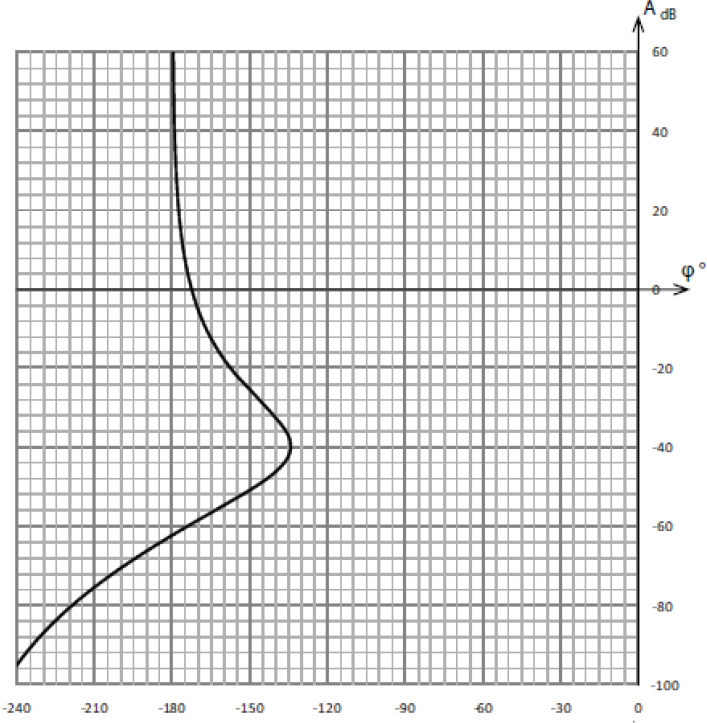
\includegraphics[width=\linewidth]{65_03}
\end{center}
\fi

\question{On donne le tracé de la réponse temporelle à un échelon de vitesse de $\SI{10}{mm.s^{-1}}$
du système corrigé pour trois valeurs de $K_V$. Quelle valeur de $K_V$ permet de valider les performances attendues
en terme de rapidité ? Donnez une valeur optimale de $K_V$ qui permette de satisfaire au mieux le cahier des
charges ? }
\ifprof
\else 
\fi

\ifprof
\else 
\begin{center}
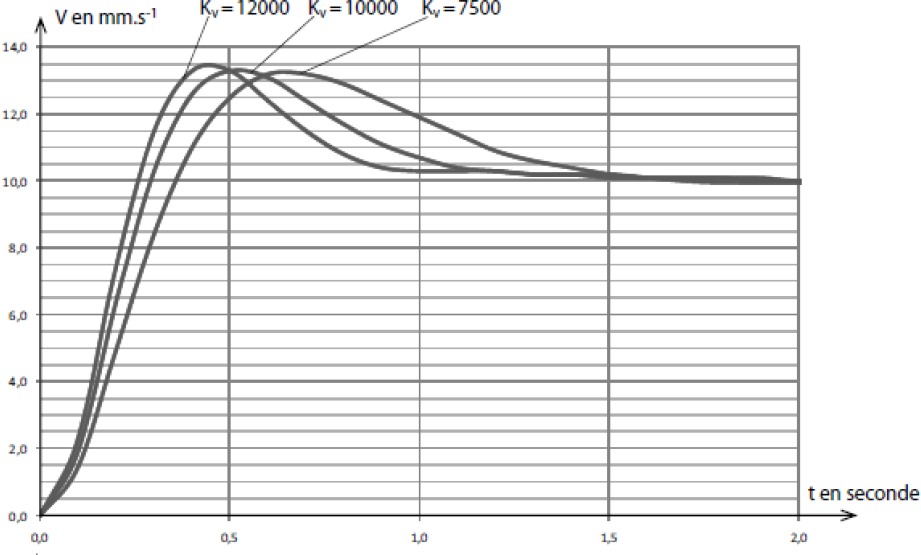
\includegraphics[width=\linewidth]{65_04}
\end{center}
\fi


\question{Le système ainsi corrigé est-il robuste aux perturbations en échelon mais également en rampe comme celles
provoquées par le système de maintien en tension ?}
\ifprof
\else 
\fi




\ifprof
\else

\noindent\footnotesize
% \fbox{\parbox{.9\linewidth}{
% Éléments de corrigé : 
% \begin{enumerate}
  % \item $\varepsilon_{\text{con \%}} = \dfrac{1}{1+K_PK_m K_{\text{pom}} K_{\text{cap}} }$;
  % \item $K_P > 19$;
  % \item $\varepsilon_{\text{pert}} = \Delta Q_e \dfrac{K_f}{1+K_{\text{cap}}K_PK_mK_{\text{pom}}}$;
  % \item $K_P > 2,19$.
  % \item $K_P < 0,125$. Il est impossible de vérifier les trois conditions avec un correcteur proportionnel.
% \end{enumerate}}}
\normalsize

\begin{flushright}
\footnotesize{Corrigé  voir \ref{C2:04:65:02}.}
\end{flushright}%
\fi